\documentclass[conference]{IEEEtran}
\IEEEoverridecommandlockouts
\usepackage{cite}
\usepackage{amsmath,amssymb,amsfonts}
\usepackage{graphicx}
\graphicspath{{../figs/}}
\usepackage{textcomp}
\usepackage{xcolor}
\usepackage{booktabs}
\usepackage{url}
\renewcommand{\topfraction}{0.95}
\renewcommand{\bottomfraction}{0.95}
\renewcommand{\textfraction}{0.05}
\renewcommand{\floatpagefraction}{0.9}
\renewcommand{\dbltopfraction}{0.95}
\renewcommand{\dblfloatpagefraction}{0.9}
\def\BibTeX{{\rm B\kern-.05em{\sc i\kern-.025em b}\kern-.08em
    T\kern-.166em\lower.7ex\hbox{E}\kern-.125emX}}

\begin{document}

\title{Clause-Activation Signatures for Attack-Family Attribution in IoMT Using Tsetlin Machines}

\author{{\small Rakesh Reddy Yakkati, Per-Arne Andersen, Rishad Shafik, Ole-Christoffer Granmo and Lei Jiao}
\thanks{Supported by the Research Council of Norway (SecureIoTM, grant 342167, TEKNOLOGIKONVER), with support from CAIR at the University of Agder, S\o rlandet Hospital Trust, and Newcastle University.}%
\thanks{R. R. Yakkati, L. Jiao, and O.-C. Granmo: Dept. of ICT, University of Agder, Grimstad, Norway; P.-A. Andersen: Dept. of Information Systems, University of Agder, Kristiansand, Norway; R. Shafik: Dept. of Microelectronic Systems, Newcastle University, UK; Contact: rakeshry@uia.no.}}

\maketitle

\begin{abstract}
%Attack-family attribution in the Internet of Medical Things (IoMT) requires accurate predictions and evidence that analysts can inspect. In this paper, we introduce Clause-Activation Signatures (CAS) to extract signed clause evidence from a trained, weighted Tsetlin Machine (WTM), which offers logically faithful explainability combined with competitive inference speed and energy efficiency compared to other deep learning approaches. Here, weight-based pruning reduces the candidate pool before complementary-pairs stability selection identifies repeatedly selected clauses. Then, averaged coefficient signs distinguish supporting from opposing evidence. To evaluate this methodology, we used the CICIoMT2024 WiFi/MQTT dataset. In the results, we observed that the full 2,400-clause TM achieves macro-F1 $0.6660\pm0.0125$, and after pruning, CAS achieves $0.6660\pm0.0316$ at $\pi_{\mathrm{thr}}=0.8$ and $0.6599\pm0.0371$ at $\pi_{\mathrm{thr}}=0.9$. Including both evidence signs, these settings use 216 and 193 distinct clauses on average, respectively. As a state-of-the-art comparison, we considered five standard classifiers using the same underlying features and achieved  $0.6284$ to $0.6733$ macro-F1. The results suggest that CAS provides a concise clause representation for IoMT attack-family attribution while maintaining predictive performance comparable to the full TM. Additionally, storing only the selected clauses may reduce memory requirements.

Attack-family attribution in the Internet of Medical Things (IoMT) requires accurate predictions while retaining a model that can be inspected and analyzed. In this paper, we propose Clause-Activation Signatures (CAS), a compact representation of a trained, weighted Tsetlin Machine (WTM) that identifies a small subset of informative clauses while preserving predictive performance. The key idea is to substantially reduce the number of clauses used by the model before performing stability-based selection. Specifically, weight-based pruning first removes clauses with limited contribution, after which complementary-pairs stability selection identifies clauses that are repeatedly selected across trained data. The signs of the averaged clause coefficients are then used to distinguish supporting from opposing evidence. We evaluate CAS on the CICIoMT2024 WiFi/MQTT dataset. The full 2,400-clause TM achieves a macro-F1 of $0.6660\pm0.0125$, while CAS achieves $0.6660\pm0.0316$ at $\pi_{\mathrm{thr}}=0.8$ and $0.6599\pm0.0371$ at $\pi_{\mathrm{thr}}=0.9$. Including both evidence signs, these settings retain only 216 and 193 distinct clauses on average, respectively, representing a substantial reduction from the original model size with little or no loss in predictive performance. For comparison, five standard classifiers using the same underlying features achieve macro-F1 scores ranging from $0.6284$ to $0.6733$. These results demonstrate that CAS can substantially simplify a WTM while maintaining competitive performance in attack-family attribution. The resulting compact clause representation reduces the storage footprint for deployment and provides a smaller, more focused set of clauses for subsequent interpretability analysis.



\end{abstract}

\begin{IEEEkeywords}
attack attribution, intrusion detection, interpretable machine learning,
IoMT, stability selection, Tsetlin Machine
\end{IEEEkeywords}

\section{Introduction and Related Work}
Attack-family attribution identifies malicious traffic types in the Internet of Medical Things (IoMT). These labels help analysts interpret security alerts, and this problem has been solved using neural network-based classifiers. For example, Yin et al.~\cite{yin2017} used recurrent neural networks to distinguish between normal traffic and four attack categories in the NSL-KDD dataset. To explain predictions, SHAP~\cite{lundberg2017shap} and LIME~\cite {ribeiro2016lime} interprets post hoc attribute contributions to input features~\cite{xaiids2025}. Deep neural network-based methods are inherently non-explainable, whereas post-hoc methods require additional software applied to an already built non-explainable model. There is a need to develop a model that is inherently explainable and able to provide analysts with insight by inspecting the detector itself.

The Tsetlin Machine (TM) learns logical conjuctive rules over Boolean
literals, which offers a lower memory footprint and interpretable, rule-based learning~\cite{granmo2018}. Weighted variants associate learned weights with clauses to obtain more compact model representations~\cite{phoulady2020}. Abeyrathna
et al.~\cite{abeyrathna2020} applied TM rules to intrusion detection on
KDD'99. Their model provided both predictions and inspectable rules.
More recently, Jaiswal et al.~\cite{jaiswal2026iomt} evaluated a TM detector on CICIoMT2024 and explained individual predictions through class-wise vote scores and clause-activation heatmaps. Also, in another study~\cite{jaiswal2026medsec}, the authors used MedSec-25 and examined feature contributions and clause activations. In addition, several datasets, such as CICIDS2017, KDD99, NSL-KDD, UNSW-NB15, and UNSW Bot-IoT, are considered, and anomaly detection is addressed using TM~\cite{10455063}. Since the TM consumes boolean data, ~\cite{jaiswal2026iomt,jaiswal2026medsec} and ~\cite{10455063} uses a $K$-bin discritizer from sklearn and a standard booleanizer from the TMU library, respectively. These studies establish both rule-based detection and
inspection of the clauses contributing to a prediction. However, previous work has not investigated how to reduce the clause pool while preserving attack-family attribution performance and identifying the most important clauses. Reducing the clause pool can ease the burden of clause-level interpretability analysis and reduce the memory required during inference.
%However, in the above contribution, there is a gap to understand the important clauses or clause removal to attain attack family attribution. 

In this paper, we introduce Clause-Activation Signatures (CAS)
to select compact, reusable class signatures from a trained clause pool. %A clause's TM vote alone does not show its additional value for distinguishing attack families. It also does not show how consistentlythe clause is selected across subsamples. In this paper, 
More specifically, a weight-based pruning first
reduces the candidate pool, and it then applies complementary-pairs stability
selection (CPSS)~\cite{meinshausen2010,shah2013} to the retained clauses'
activations. Further, averaged coefficients from
one-versus-rest models identify supporting and opposing evidence for
each class. These evidence signs are estimated separately from the
original TM voting signs. CAS scores each flow by normalizing the signed
evidence from selected clauses that activate.
We evaluate whether CAS reduces the evidence set while retaining
predictive performance. %Our evaluation uses per-class sampling caps without SMOTE and separate partitions for TM fitting, signature extraction, and operating-point selection. 
%This sampling and partitioning protocol differs from the prior CICIoMT2024 work~\cite{jaiswal2026iomt}. The caps also change the test class distribution. This can affect macro-F1 through per-class precision, despite equal class weighting. These differences prevent a direct performance ranking against their published results. We therefore compare CAS with the full TM and standard classifiers evaluated within this study on a common report set.

The main contributions include the following aspects:
\begin{itemize}
\item A clause-based attribution layer that combines CPSS with signed,
normalized evidence to construct reusable class signatures.
\item A sufficient margin condition for prediction-preserving TM pruning
and an explicit account of the scope of CPSS error control.
\end{itemize}

\begin{figure*}[!t]
\centering

\includegraphics[width=1\textwidth]{fig_cpss_protocol.pdf}
\caption{CAS pipeline with disjoint TM-fit, CPSS-fit, selection, and
report partitions.}
\label{fig:cpss}
\end{figure*}

\section{Method: Clause-Activation Signatures}
\subsection{Booleanisation and Weighted TM}
\label{sec:bool}
Figure~\ref{fig:cpss} summarizes the pipeline. Since the TM consumes boolean data,~\cite{jaiswal2026iomt,jaiswal2026medsec} and~\cite{10455063} use a $K$-bin discritizer from sklearn and a standard booleanizer from the TMU library, respectively. In this paper, training-fitted quantile
bins encode numeric features as cumulative thermometer bits (non-finite
values are replaced with the finite training maximum). %TMU~\cite{tmu} supplies literal negation internally. 

For $N_{\mathrm{cls}}$ classes indexed by $c\in\{1,\dots,N_{\mathrm{cls}}\}$ and $C$ clauses per class indexed by $j\in\{1,\dots,C\}$, the trained pool produces Boolean activations
$z_{c,j}(x)$ and signed class sums
\begin{equation}
 f_c(x)=\sum_{j=1}^{C} w_{c,j}z_{c,j}(x),\qquad
 \hat y_{\mathrm{TM}}(x)=\arg\max_c f_c(x).
 \label{eq:tm}
\end{equation}
Flattening class and clause indices gives the activation matrix
$Z\in\{0,1\}^{n\times p}$ over $n$ samples (flows), initially with $p=N_{\mathrm{cls}}C$.



\subsection{Clause-Pool Pruning}
\label{sec:prune}
Let $m_{c,j}\in\{0,1\}$ retain a clause and
$f_c(x;m)=\sum_j m_{c,j}w_{c,j}z_{c,j}(x)$. The target is a small
pool whose macro-F1 on the selection partition remains within
$\varepsilon$ of the full model:
\begin{equation}
 \min_m\|m\|_0\quad\text{s.t.}\quad
 F_{1,\mathrm{sel}}(m)\ge F_{1,\mathrm{sel}}(\mathbf1)-\varepsilon.
 \label{eq:prune}
\end{equation}
We use a magnitude surrogate instead of solving this discrete objective.
For removed indices $D_c$, set
$R_c=\sum_{j\in D_c}|w_{c,j}|$ and $R=\max_cR_c$.
Since activations are Boolean,
\begin{equation}
 |f_c(x)-f_c(x;m)|\le R_c\le R.
 \label{eq:perturb}
\end{equation}
If $a=\hat y_{\mathrm{TM}}(x)$ and
$\gamma(x)=f_a(x)-\max_{c\ne a}f_c(x)$, the margin of $a$ over any
competing class decreases by at most $2R$. Thus
\begin{equation}
 \gamma(x)>2R\quad\Longrightarrow\quad
 \arg\max_c f_c(x;m)=\hat y_{\mathrm{TM}}(x).
 \label{eq:margin}
\end{equation}
For a fixed deletion budget $k$ per class, the smallest-magnitude
weights minimize this surrogate:
\begin{equation}
 D_c^*(k)=\operatorname{arg\,min}_{|D|=k}
                   \sum_{j\in D}|w_{c,j}|.
 \label{eq:greedy}
\end{equation}


\subsection{CPSS and Signed Evidence}
\label{sec:cpss}
For each class $\ell$, CPSS divides the fit partition into $B$
Complementary pairs as shown in Fig~1. On each of the $2B$ halves, a class-balanced
$\ell_1$ logistic model predicts the one-versus-rest class label from
$Z$. For half $h$ and inverse-regularisation strength
$\kappa\in\Lambda$, let $\beta_{\ell j}^{h,\kappa}$ be the fitted
coefficient. A clause receives one vote if any grid point selects it,
using numerical tolerance $\delta$:
\begin{equation}
 \hat\pi_{\ell j}=\frac{1}{2B}\sum_{h=1}^{2B}
 \mathbf1\!\left\{\max_{\kappa\in\Lambda}
             |\beta_{\ell j}^{h,\kappa}|>\delta\right\}.
 \label{eq:stability}
\end{equation}
Let $\bar\beta_{\ell j}$ average coefficients over all halves and grid points, including zeros. The signed supports are
\begin{equation}
 S_\ell^\pm=\{j:\hat\pi_{\ell j}\ge\pi_{\mathrm{thr}},\quad
                                  \pm\bar\beta_{\ell j}>0\}.
 \label{eq:sign}
\end{equation}
Positive coefficients provide inculpatory evidence; negative ones provide exculpatory evidence. The attribution rule is
\begin{equation}
 s_\ell(x)=\frac{\sum_{j\in S_\ell^+}\hat\pi_{\ell j}z_j(x)
                 -\sum_{j\in S_\ell^-}\hat\pi_{\ell j}z_j(x)}
                {\sum_{j\in S_\ell^+}\hat\pi_{\ell j}}.
 \label{eq:score}
\end{equation}
Prediction uses $\hat y(x)=\arg\max_\ell s_\ell(x)$.

\subsection{Scope of Stability Error Control}
\label{sec:cert}
For a fixed pool and selector, let $p_j$ denote a clause's population
selection probability on a half-sample, $L_\theta=\{j:p_j\le\theta\}$,
and $q$ the expected number selected per half. Under the sampling
conditions of CPSS~\cite{shah2013}, the sign-agnostic support $S_\ell$
satisfies, for $\pi_{\mathrm{thr}}>1/2$,
\begin{equation}
 \mathbb E|S_\ell\cap L_\theta|
 \le\frac{\theta q}{2\pi_{\mathrm{thr}}-1}.
 \label{eq:bound}
\end{equation}
Taking $\theta=q/p$ yields $q^2/((2\pi_{\mathrm{thr}}-1)p)$.
This controls low-selection-probability inclusions. Interpreting them as false discoveries requires additional assumptions, using
$\hat q=\sum_j\hat\pi_{\ell j}$ is a plug-in diagnostic, not a validated false-discovery certificate. Correlated flows, adaptive
operating-point selection, and coefficient signs require separate
consideration. No finite bound is claimed at $\pi_{\mathrm{thr}}=0.5$.

\section{Experimental Setup and Results}
\label{sec:setup}
\subsection{Dataset Details}
CICIoMT2024 contains 18 attacks on 40 devices, including 25 real
and 15 simulated devices~\cite{dadkhah2024}. We use its WiFi/MQTT
flow features with six labels: Benign, DDoS, DoS, MQTT, Recon, and
Spoofing. The selected features exclude IP addresses and port fields.
Sampling is capped at 40,000 training and 15,000 test rows per class.
The training set contains 195,338 rows (19,291 Benign, 16,047
Spoofing, 40,000 in each remaining class). Meanwhile, the test set contains
80,868 rows (5,868 Spoofing and 15,000 in each other class). Using this data, a stratified split of the training set creates 136,735 TM-fit rows,
39,068 CPSS-fit rows and 19,535 selection rows. The test set serves
as the report set for final evaluation. The TM remains frozen during
signature extraction, and the CPSS-fit flows are withheld from TM
training.
\subsection{TM parameters and hyperparameter optimization}
The TM-based booleanizer encodes each feature into bit vectors using quantile-based thresholds. Hence,
the 22 numeric features use up to ten quantile bins, giving a cached
154-bit representation that includes redundant bits from repeated
quantiles. The TM hyperparameter used in this work is $C=400$ clauses per class (200 positive and
200 negative), $T=320$, $s=8$, and 25 epochs.
CPSS uses class-balanced liblinear fits with 200 maximum iterations,
$\delta=10^{-8}$, and $\Lambda=\operatorname{geomspace}(0.001,0.1,6)$.
Pruning sweeps $k\in\{0,5,\ldots,395\}$ with $\varepsilon=0.01$.
For each pool, the operating point $(B,\pi_{\mathrm{thr}})$ is chosen
to maximize mean selection macro-F1 over
$B\in\{5,10,15,20,25\}$ and
$\pi_{\mathrm{thr}}\in\{0.5,0.6,0.7,0.8,0.9\}$.

\subsection{Closed-Set Attribution and Sign Validation}
\label{sec:taska}\label{sec:validation}
Table~\ref{tab:headline} compares predictive performance and evidence
size. For CAS, size is the mean positive-evidence support summed across
classes. It excludes opposing evidence, and a clause selected for
multiple classes is counted in each class's support.

For the pruned pool, the selection-set macro-F1 chooses
$(B,\pi_{\mathrm{thr}})=(10,0.5)$. This setting achieves report-set
macro-F1 $0.6755$ with 190 positive-evidence clauses. We also highlight $(5,0.8)$ and $(10,0.9)$ to illustrate the
trade-off at higher selection thresholds and smaller positive supports.
At $(5,0.8)$, CAS uses 149 positive-evidence clauses and matches the full TM's mean macro-F1 to the reported precision. At
$\pi_{\mathrm{thr}}=0.9$, this count falls to 126 and mean macro-F1
decreases by $0.0061$, less than the reported standard deviations
across seeds. Including opposing evidence, these two settings use
216 and 193 distinct clauses on average: $11.1$--$12.4$ times fewer
than the full pool. Their summed positive/negative supports are
149/199 and 126/173, respectively. Clauses shared across classes explain
why the distinct counts are smaller than these sums. The selected $(10,0.5)$ setting uses 251 distinct signed clauses. All counts are
rounded means over three seeds. Figure~\ref{fig:frontier} plots the trade-off using positive-support counts.

Two ablations examine what makes the selected evidence useful.
Replacing clause activations with the 154 input literals under the
same readout yields macro-F1 $0.5876\pm0.0112$. This result supports
the value of the clauses' conjunctive structure. A sign-agnostic scorer
normalizes the stability-weighted sum over all selected clauses.
It yields macro-F1 $0.025\pm0.032$. This drop shows that the readout
depends on distinguishing supporting from opposing evidence.

\begin{table}[t]
\centering
\caption{Report-set performance (three seeds). Clause counts denote
TM pool size or CAS positive supports summed across classes.}
\label{tab:headline}
\footnotesize
\setlength{\tabcolsep}{1pt}
\begin{tabular}{@{}lcccc@{}}
\toprule
Method & $(B,\pi_{\mathrm{thr}})$ & Clauses & macro-F1 & Accuracy \\
\midrule
TM, full pool & --- & 2{,}400 & $0.6660\pm0.0125$ & 0.7033 \\
TM, pruned pool & --- & 360 & $0.6615\pm0.0115$ & 0.6982 \\
CAS, full pool & $(10,0.9)$ & 154 & $0.6408\pm0.0168$ & 0.6676 \\
CAS, pruned pool & $(10,0.9)$ & $\mathbf{126}$ & $0.6599\pm0.0371$ & 0.6972 \\
CAS, pruned pool & $(5,0.8)$ & 149 & $0.6660\pm0.0316$ & 0.7037 \\
CAS, pruned pool & $(10,0.5)$ & 190 & $\mathbf{0.6755\pm0.0183}$ & 0.7126 \\
\midrule
Input literals, same readout & $(10,0.9)$ & --- & $0.5876\pm0.0112$ & 0.6271 \\
\bottomrule
\end{tabular}
\end{table}

\subsection{Comparison with Standard Classifiers}
\label{sec:baselines}
Table~\ref{tab:baselines} compares CAS with five standard classifiers. All the baselines are also provided with the same dataset as presented in Section~IIIA. 
%Each baseline receives the 22 numeric features in their original continuous form. The TM uses thermometer encoding. We fit all baselines on the union of the TM-fit and CPSS-fit partitions. This gives them the175,803 labelled rows CAS uses across its two stages. 
We choose
hyperparameters on the selection partition and evaluate each model once
on the report set. The 300-tree random
forest~\cite{breiman2001} has the highest mean macro-F1 among these
baselines, $0.6733$.
XGBoost follows at $0.6640$, the decision tree at $0.6526$, the
binarized neural network at $0.6503$, and the $\ell_1$ linear model at
$0.6284$. Standard deviations across seeds are below $0.002$ for the
tree models, $0.011$ for the linear model, and $0.043$ for the BNN.
XGBoost gives identical results across seeds in this experiment. It uses no row or column subsampling. 

The binarized neural network~\cite{hubara2016bnn} provides a neural
comparison that uses bitwise operations, as does the TM.
It is important to note that the BNN reaches $0.6503$ using 106,496 binary weights. Meanwhile, CAS attains
$0.6660$ from 216 distinct signed clauses. These counts describe
different model components as they do not establish relative memory or
runtime costs.

%These baselines provide several points of comparison. A single decision tree and an $\ell_1$ linear model serve as interpretable references.
%Bagged and boosted tree ensembles provide black-box references.





\begin{table}[t]
\centering
\caption{Standard classifiers on the 22 numeric features, three-seed
means on the report set.}
\label{tab:baselines}
\footnotesize
\setlength{\tabcolsep}{3pt}
\begin{tabular}{@{}lcc@{}}
\toprule
Model & macro-F1 & Accuracy \\
\midrule
Random forest~\cite{breiman2001} & $\mathbf{0.6733}$ & 0.7251 \\
XGBoost~\cite{chen2016xgboost} & $0.6640$ & 0.7112 \\
Decision tree & $0.6526$ & 0.6972 \\
Binarized neural network~\cite{hubara2016bnn} & $0.6503$ & 0.6697 \\
$\ell_1$ logistic regression~\cite{tibshirani1996} & $0.6284$ & 0.6465 \\
\bottomrule
\end{tabular}
\end{table}

\begin{figure}[t]
\centering
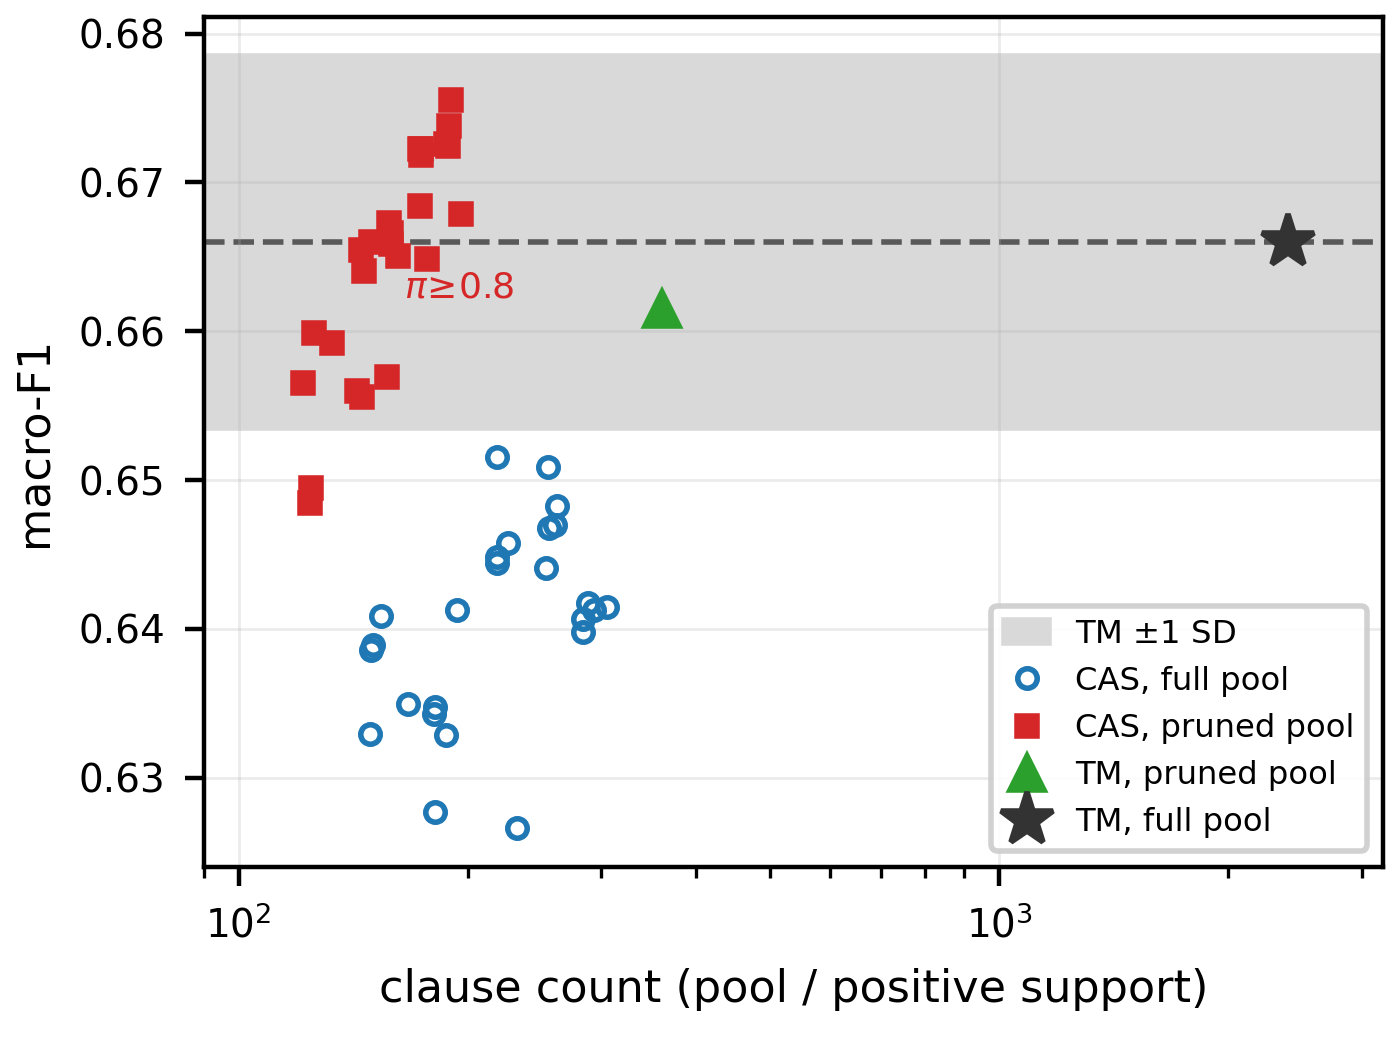
\includegraphics[width=0.9\columnwidth]{fig_signature_frontier.png}
\caption{CAS size--performance trade-off. The band is TM mean$\pm$SD;
23 of 25 pruned-pool settings lie within it.}
\label{fig:frontier}
\end{figure}

\subsection{Sensitivity Before and After Pruning}
\label{sec:sweep}
To assess sensitivity to the CPSS settings, we vary the selection
threshold and pair count. At $B=15$, sweeping $\pi_{\mathrm{thr}}$ over
$\{0.5,\ldots,0.9\}$ spans macro-F1 0.656--0.674 on the pruned pool and
0.633--0.652 on the full pool. At $\pi_{\mathrm{thr}}=0.8$, varying $B$ from 5 to 25 gives ranges of 0.656--0.666 and 0.628--0.641, respectively. Fig.~\ref{fig:sweep} compares these sweeps with the
pruned-TM baselines. In these sweeps, CAS performs better when selection
starts from the pruned pool. This suggests that removing low-weight clauses helps signature extraction in this setting. Across the
pruned-pool operating points, positive-evidence support sizes range
from 122 to 196 (Fig.~\ref{fig:frontier}).

\begin{figure}[t]
\centering
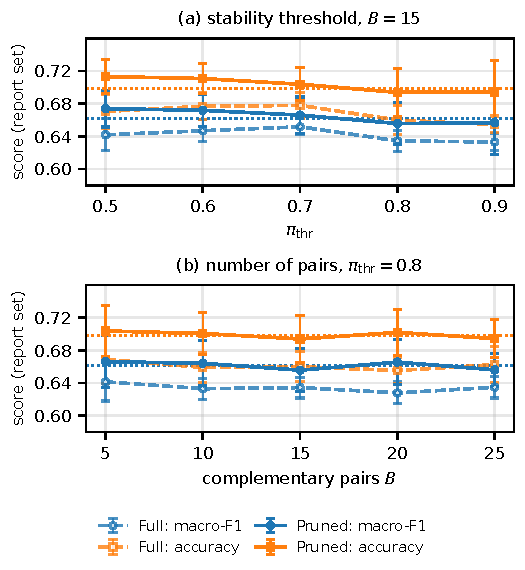
\includegraphics[width=\columnwidth]{fig_sweep_heldout.pdf}
\caption{CAS sensitivity (three-seed mean$\pm$SD): (a) threshold at
$B=15$; (b) pair count at $\pi_{\mathrm{thr}}=0.8$. Dotted lines: pruned TM.}
\label{fig:sweep}
\end{figure}


\subsection{Pruning and Signature Size}
\label{sec:pruned}\label{sec:signatures}
To examine the effect of pruning alone, Fig.~\ref{fig:pruning} shows
TM performance across removal budgets. Report-set macro-F1 and
accuracy remain approximately steady as the pool shrinks
from 2,400 to roughly 360 clauses, then decline with further removal.
Using only the selection partition to choose the pruning budget gives
$k^*=340$. This leaves 60 clauses per class and 360 in total,
a reduction of $85\%$. At that budget, the pruned TM achieves macro-F1
$0.6615\pm0.0115$ against $0.6660\pm0.0125$ for the full pool
(Table~\ref{tab:headline}). Pruning therefore removes most of the
pool with a mean macro-F1 decrease of $0.0045$.

\begin{figure}[t]
\centering
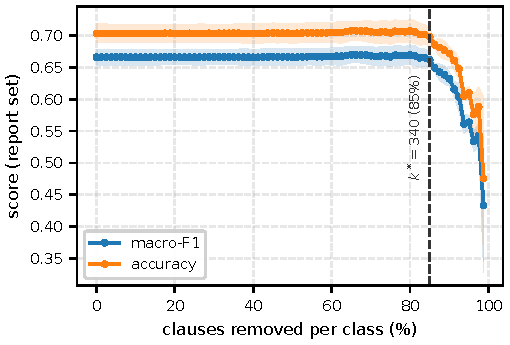
\includegraphics[width=0.92\columnwidth]{fig_clause_pruning_heldout.pdf}
\caption{Pruning sensitivity (mean$\pm$SD); the dashed line marks
$k^*=340$, chosen on the selection set.}
\label{fig:pruning}
\end{figure}

Table~\ref{tab:reduction} shows both evidence signs at each pool's
selected setting for seed 42. Summed positive/negative supports are
150/585 for the full pool and 185/233 after pruning.
These CAS signs are estimated from the pooled clauses across all six
classes and differ from the original TM polarities. Shared clauses
are counted in each class. The selected thresholds differ, so pruning
need not reduce the summed supports.

\begin{table}[t]
\centering
\caption{CAS supports, seed 42: full $(10,0.9)$; pruned $(10,0.5)$.}
\label{tab:reduction}
\footnotesize
\begin{tabular}{@{}lrrrr@{}}
\toprule
& \multicolumn{2}{c}{Full pool} & \multicolumn{2}{c}{Pruned pool} \\
\cmidrule(lr){2-3}\cmidrule(l){4-5}
Class & $|S^+|$ & $|S^-|$ & $|S^+|$ & $|S^-|$ \\
\midrule
Benign & 21 & 65 & 35 & 37 \\
DDoS & 29 & 130 & 29 & 39 \\
DoS & 21 & 180 & 38 & 40 \\
MQTT & 21 & 67 & 17 & 20 \\
Recon & 19 & 47 & 27 & 54 \\
Spoofing & 39 & 96 & 39 & 43 \\
\midrule
Total & 150 & 585 & 185 & 233 \\
\bottomrule
\end{tabular}
\end{table}

\section{Conclusion}
%CAS extracts reusable, signed clause evidence for IoMT attack-family attribution. On capped CICIoMT2024 data, pruning removes $85\%$ of the TM pool. CAS matches the full TM's mean macro-F1 of $0.6660$ with 216 distinct signed clauses. Using 193 yields $0.6599$. Ablations support the use of conjunctive rules and evidence signs. Both highlighted settings fall within the baseline performance range. Their compact evidence traces to the selected clauses. The pruning bound depends on the stated margin condition. Under its sampling assumptions, CPSS controls low-selection-probability inclusions, without certifying false discoveries or signs. Further datasets, analyst studies, and runtime measurements are needed to assess generalization, explanation value, and deployment savings.

In this paper, we introduced CAS for compact, signed clause-based attribution of IoMT attacks. By combining weight-based pruning with complementary-pairs stability selection, CAS reduces a 2,400-clause TM to 216 distinct signed clauses while matching its macro-F1 of 0.6660. Further increasing the selection threshold reduces the representation to 193 clauses, with macro-F1 decreasing slightly to 0.6599. These results show that substantial clause reduction is possible with little loss in predictive performance in this application. Ablations further support the use of conjunctive clauses and signed evidence. The theoretical results for pruning and stability selection hold under their stated assumptions, while further evaluation on additional datasets is needed to assess generalization to other applications.


\bibliographystyle{IEEEtran}
\bibliography{CAS_4page}
\end{document}
